\documentclass[12pt]{article}
\usepackage{amsmath}
\usepackage{graphicx}
\usepackage{float}
\usepackage{hyperref}
\usepackage{geometry}
\usepackage{minted}
\geometry{a4paper, margin=1in}

\hypersetup{
    colorlinks=true,
    linkcolor=cyan,
    filecolor=magenta,      
    urlcolor=blue,
}

\begin{document}

\begin{titlepage}
    \centering
    \vspace*{1in}
    
    \large
    \textbf{Tweet Sentiment Analysis: Comparing SVM, CNN/RNN, and BERT Models}

    \text{
    \vspace{0.5in}
    30562 - Machine Learning and Artificial Intelligence
    }
    
    \vspace{0.5in}
    Mark Maci \\
    \texttt{mark.maci@studbocconi.it} \\
    3296048\\
    
    \vspace{0.5in}
    Cedric Bellens \\
    \texttt{email} \\
    id \\

    \vspace{0.5in}
    Katarina Litricin \\
    \texttt{email} \\
    id \\
    
    \vspace{0.5in}
    Anil Egin \\
    \texttt{email} \\
    id \\
    
    \vfill
    \large
    \today
    
\end{titlepage}

\begin{abstract}
This paper presents a comparative study of tweet sentiment analysis using three different types of models: Support Vector Machine (SVM), Convolutional/Recurrent Neural Networks (CNN/RNN), and Bidirectional Encoder Representations from Transformers (BERT). Each model represents a different era of technological advancement in machine learning. The study employs various feature extraction techniques, including TF-IDF and GloVe embeddings for SVM, and more advanced methods for CNN/RNN and BERT models. By evaluating the performance of these models on a standardized dataset, we aim to highlight the progression and effectiveness of different machine learning approaches in sentiment analysis.
\end{abstract}
    
\section{Introduction}
Sentiment analysis, also known as opinion mining, is a crucial task in the language understanding realm of natural language processing (NLP) that involves determining the sentiment expressed in a piece of text. With the rise of social media platforms like Twitter, sentiment analysis has become an invaluable tool for understanding public opinion, tracking market trends, and monitoring social phenomena. \\

The applications of sentiment analysis are extensive. Businesses utilize it to gauge customer satisfaction and manage brand reputation by analyzing feedback from social media, reviews, and surveys. Governments and political analysts monitor public sentiment to assess the impact of policies and public statements. In the financial sector, sentiment analysis helps predict stock market trends by analyzing news and social media sentiment. Healthcare providers use it to monitor patient feedback and improve services.\\

Given the variety of models and techniques available for sentiment analysis, this study aims to compare the performance of three distinct types of models: Support  Vector Machine (SVM), Convolutional/Recurrent Neural Networks (CNN/RNN), and Bidirectional Encoder Representations from Transformers (BERT). These models represent different stages of advancement in machine learning, somewhat analogous to comparing different generations of cars - from classic models to modern high-performance vehicles.\\

The focus of this study is not only on the models themselves but also on the feature extraction techniques used across them to gain a better understanding on how these models leverage different types of data representations. Specifically, we will compare the use of TF-IDF and GloVe embeddings, tokenization and lemmatization techniques, and other preprocessing steps that are essential for effective sentiment analysis.\\


\section{Related Work}
Sentiment analysis has been a prominent area of research in natural language processing (NLP) for several years. Various approaches have been developed, ranging from traditional machine learning methods to advanced deep learning techniques.

\subsection{Traditional Machine Learning Approaches}
Traditional machine learning techniques, such as Support Vector Machines (SVM) and Naive Bayes, have been widely used for sentiment analysis. \href{https://www.cs.cornell.edu/home/llee/papers/sentiment.pdf}{Pang et al. (2002)} employed SVMs for sentiment classification of movie reviews and demonstrated the effectiveness of SVMs in handling high-dimensional feature spaces typical of text data. These models often rely on feature extraction techniques like Term Frequency-Inverse Document Frequency (TF-IDF) to transform text into numerical vectors.

\subsection{Deep Learning Approaches}
In recent years, deep learning methods have significantly advanced the field of sentiment analysis. Convolutional Neural Networks (CNNs) and Recurrent Neural Networks (RNNs) have been particularly successful. \href{https://arxiv.org/abs/1408.5882}{Kim (2014)} introduced a CNN architecture for sentence classification that achieved remarkable results by leveraging word embeddings and convolutional layers to capture local and global features of text. Similarly, RNNs, especially Long Short-Term Memory (LSTM) networks, have been effective in modeling sequential data and capturing long-term dependencies in text, as shown by \href{https://www.aclweb.org/anthology/P15-1067/}{Tang et al. (2015)} in their work on sentiment analysis.

\subsection{Transformers and Pre-trained Models}
The advent of transformer models and pre-trained language representations has revolutionized sentiment analysis. The Bidirectional Encoder Representations from Transformers (BERT) model, introduced by \href{https://arxiv.org/abs/1810.04805}{Devlin et al. (2019)}, has set new benchmarks in various NLP tasks, including sentiment analysis. BERT's ability to understand context from both directions in a sentence allows it to capture nuanced sentiment information that traditional and deep learning models might miss.

\subsection{Feature Extraction Techniques}
Feature extraction is a critical step in sentiment analysis, impacting the performance of the model significantly. Traditional methods like TF-IDF and Bag of Words (BoW) are still relevant and widely used for simpler models like SVMs. However, with the rise of deep learning, word embeddings such as Word2Vec, introduced by \href{https://arxiv.org/abs/1301.3781}{Mikolov et al.}, GloVe, introduced by \href{https://nlp.stanford.edu/pubs/glove.pdf}{Pennington et al. (2014)}, and contextual embeddings like those used in BERT have become the standard for representing text in a more meaningful way.


\section{Methodology}

\subsection{Data Collection and Preprocessing}
For this study, we use the Sentiment140 dataset, which consists of 1.6 million tweets. This dataset is particularly valuable for sentiment analysis as it provides a large volume of data that is crucial for training machine learning models. The Sentiment140 dataset was introduced by \href{https://cs.stanford.edu/people/alecmgo/papers/TwitterDistantSupervision09.pdf}{Go et al. (2009)} in their paper "Twitter Sentiment Classification using Distant Supervision."

The dataset was created using a distant supervision approach, which leverages emoticons as noisy labels to automatically classify the sentiment of tweets. Emoticons such as ":)" and ":(" were used to identify positive and negative sentiments, respectively. This method allows for the collection of a large, labeled dataset without manual annotation. The dataset includes tweets labeled as positive (4), negative (0), or neutral (2).

The dataset can be conveniently accessed and loaded into our analysis environment using the Huggingface \texttt{datasets} module. 


\subsection{Feature Extraction}
Various feature extraction techniques are employed to convert the raw text data into numerical vectors that can be used as input to the machine learning models. These techniques include:
\begin{itemize}
    \item \textbf{TF-IDF}: A numerical statistic intended to reflect the importance of a word in a document relative to a corpus.
    \item \textbf{GloVe}: Global Vectors for Word Representation, which creates word embeddings by aggregating global word-word co-occurrence statistics from a corpus.
    \item \textbf{Tokenization and Lemmatization}: The process of breaking down text into individual words (tokens) and reducing them to their base or root form (lemmas).
    \item \textbf{Preprocessing}: Steps such as removing stopwords, punctuation, and special characters, as well as lowercasing the text.
\end{itemize}

\subsection{Support Vector Machine (SVM)}
SVM is a supervised learning model used for classification tasks. It works by finding the hyperplane that best separates the classes in the feature space. Rather than using a prewritten model from a library, we implement the SVM model from scratch to gain a deeper understanding of its inner workings. The SVM model is trained using the features extracted from the tweet dataset and evaluated based on performance metrics such as accuracy, precision, recall, and F1-score.

\subsubsection{Mathematical Formulation}
The SVM optimization problem can be formulated as follows:
\begin{align}
\min_{\mathbf{w}, b} & \quad \frac{1}{2} \|\mathbf{w}\|^2 + C \sum_{i=1}^{n} \max(0, 1 - y_i (\mathbf{w} \cdot \mathbf{x}_i + b)) \\
\text{subject to} & \quad y_i (\mathbf{w} \cdot \mathbf{x}_i + b) \geq 1 - \xi_i, \quad \xi_i \geq 0
\end{align}

corresponding to the following code snippet:

\begin{minted}{python}
for batch_start in range(0, n_samples, self.batch_size):
    for j in range(batch_start, min(batch_start + self.batch_size, n_samples)):
        idx = ids[j]
        condition = Y[idx] * (np.dot(X[idx], self.w) + self.b) >= 1
        if not condition:
            grad_w += self.C * Y[idx] * X[idx]
            grad_b += self.C * Y[idx]

    self.w -= self.lr * (2 * self.w - grad_w)
    self.b += self.lr * grad_b
\end{minted}

\subsubsection{Implementation Details}
The SVM implementation includes a custom SVM class with methods for fitting the model and making predictions. The hinge loss function is defined as:

\begin{equation}
L(\mathbf{w}, b) = \frac{1}{2} \|\mathbf{w}\|^2 + C \sum_{i=1}^{n} \max(0, 1 - y_i (\mathbf{w} \cdot \mathbf{x}_i + b))
\end{equation}

\begin{minted}{python}
def hingeloss(self, w, b, X, Y):
        loss = 0.5 * np.dot(w, w.T)
        for i in range(X.shape[0]):
            ti = Y[i] * (np.dot(X[i], w.T) + b)
            loss += self.C * max(0, 1 - ti)
        return loss
\end{minted}

The training process uses gradient descent with batch processing. The hyperparameters are set as follows: $C=1.0$, learning rate $=0.001$, epochs $=50$, batch size $=100$.

\section{Experimental Results}

\subsection{SVM Model Performance}
The SVM model is trained using TF-IDF and lemmatization features. The model is evaluated on the test set using metrics such as accuracy, precision, recall, and F1-score. The results are visualized in Figure \ref{fig:accuracy} and summarized in Table \ref{tab:classification_report}

\begin{table}[H]
    \centering
    \begin{tabular}{lcccc}
    \hline
    Class & Precision & Recall & F1-Score & Support \\
    \hline
    -1 & 0.74 & 0.86 & 0.80 & 159494 \\
    1 & 0.84 & 0.69 & 0.76 & 160506 \\
    \hline
    Accuracy & \multicolumn{4}{c}{0.77931875} \\
    Macro Avg & 0.79 & 0.78 & 0.78 & 320000 \\
    Weighted Avg & 0.79 & 0.78 & 0.78 & 320000 \\
    \hline
    \end{tabular}
    \caption{Classification Report for SVM Model}
    \label{tab:classification_report}
    \end{table}

\begin{figure}[H]
    \centering
    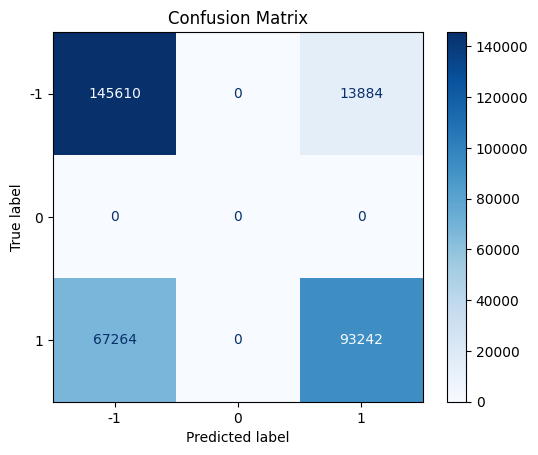
\includegraphics[width=0.6\textwidth]{svm_50epoch_tfidf.png}
    \caption{Confusion Matrix for SVM Model}
    \label{fig:accuracy}
\end{figure}

\subsection{CNN Model Performance}
The CNN model is trained using only tokenization and lemmatization features. The model's performance is evaluated on the test set, and the results are visualized in the following figures.

\begin{figure}[H]
    \centering
    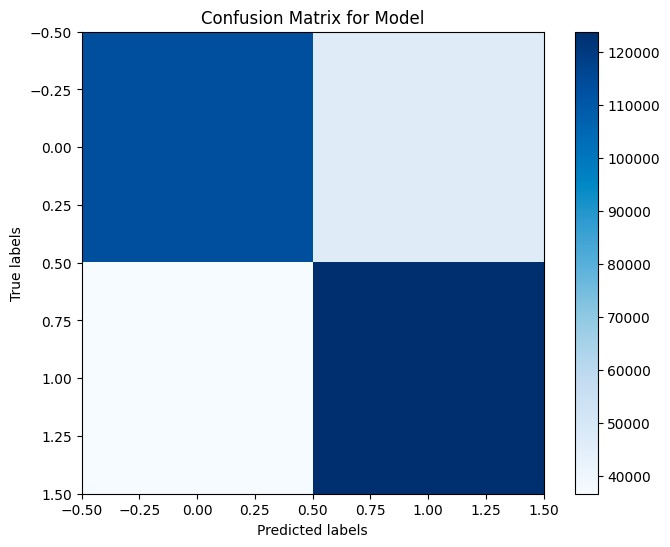
\includegraphics[width=0.6\textwidth]{WhatsApp Image 2024-05-29 at 02.36.54 (1).jpeg}
    \caption{Confusion Matrix for CNN Model}
    \label{fig:cnn_confusion_matrix}
\end{figure}

\begin{figure}[H]
    \centering
    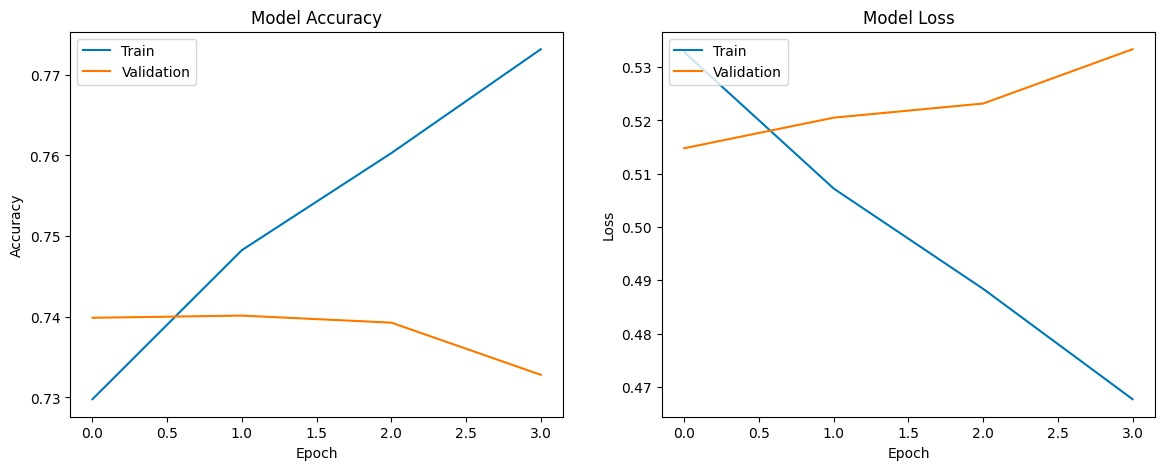
\includegraphics[width=0.8\textwidth]{WhatsApp Image 2024-05-29 at 02.37.14.jpeg}
    \caption{Training and Validation Accuracy/Loss for CNN Model}
    \label{fig:cnn_training_validation}
\end{figure}

\begin{table}[H]
    \centering
    \begin{tabular}{lcccc}
    \hline
    Class & Precision & Recall & F1-Score & Support \\
    \hline
    0 & 0.76 & 0.71 & 0.73 & 159494 \\
    1 & 0.73 & 0.77 & 0.75 & 160506 \\
    \hline
    Accuracy & \multicolumn{4}{c}{0.740409375} \\
    Macro Avg & 0.74 & 0.74 & 0.74 & 320000 \\
    Weighted Avg & 0.74 & 0.74 & 0.74 & 320000 \\
    \hline
    \end{tabular}
    \caption{Classification Report for CNN Model}
    \label{tab:cnn_classification_report}
\end{table}


\section{Discussion}
The SVM model's performance is interpreted in the context of tweet sentiment classification. A brief comparison with CNN/RNN and BERT models is provided, highlighting the strengths and limitations of the SVM model.

\section{Conclusion}
The SVM model, when combined with TF-IDF and GloVe features, shows effective performance in tweet sentiment analysis. Future work could explore the use of more advanced embeddings and hyperparameter tuning to improve results.

\section*{References}
\bibliographystyle{plain}
\bibliography{references}

\appendix
\section{Code Snippets}
Additional code snippets and detailed tables can be found here.

\end{document}
